\chapter{RSHub-agent: Software Components, Architecture, and API Specification}

% ============================================
% Section 1: Software Components and Dependencies
% ============================================
\section{Software Components and Dependencies}
This section records the concrete software stack used in the current implementation, so that deployment assumptions and runtime behavior are traceable.

\subsection{Project Technology Stack Overview}

RSHub-agent adopts a modular microservices architecture consisting of three main sub-projects:

\begin{table}[H]
	\centering
	\caption{Project Composition Overview}
	\begin{tabular}{@{}lll@{}}
		\toprule
		\textbf{Sub-project} & \textbf{Technology Stack} & \textbf{Purpose} \\
		\midrule
		RSHub-agent-main & Python + FastAPI & AI Agent backend service \\
		RSHub-web-main & React + Docusaurus & Frontend website \\
		RSHub-gitsync-main & Python & Git synchronization tool \\
		\bottomrule
	\end{tabular}
\end{table}

\subsection{Backend Technology Components}

\begin{longtable}{@{}p{3.5cm}p{2.5cm}p{7.5cm}@{}}
	\caption{Backend Components Inventory} \\
	\toprule
	\textbf{Component} & \textbf{Version} & \textbf{Description} \\
	\midrule
	\endfirsthead
	\multicolumn{3}{c}{\tablename\ \thetable{} -- Continued} \\
	\toprule
	\textbf{Component} & \textbf{Version} & \textbf{Description} \\
	\midrule
	\endhead
	\bottomrule
	\endfoot
	FastAPI & $\geq$0.115.0 & High-performance Python web framework for RESTful APIs \\
	Uvicorn & $\geq$0.32.0 & ASGI server supporting HTTP/1.1 and WebSocket \\
	Pydantic & $\geq$2.0.0 & Data validation and serialization library \\
	Pydantic Settings & $\geq$2.0.0 & Configuration management with env variable support \\
	HTTPX & Latest & Async HTTP client supporting HTTP/1.1 and HTTP/2 \\
	Requests & Latest & Classic synchronous HTTP library \\
	OpenAI SDK & $\geq$1.0.0 & Official OpenAI Python SDK for LLM calls \\
	Jinja2 & $\geq$3.1.0 & Template engine for dynamic prompt generation \\
	NumPy & $\geq$1.24.0 & Scientific computing with multi-dimensional arrays \\
	Matplotlib & $\geq$3.7.0 & Data visualization for plotting results \\
	Scikit-image & $\geq$0.25.2 & Image processing for remote sensing analysis \\
	RSHub & $\geq$0.3.5 & Core microwave remote sensing library (DMRT, NMM3D) \\
	PyYAML & Latest & YAML parsing for Skill definition files \\
	Python-dotenv & Latest & Environment variable loading from .env files \\
	UV & Latest & Modern Python package manager \\
\end{longtable}

\subsection{Frontend Technology Components}

\begin{longtable}{@{}p{3.5cm}p{2.5cm}p{7.5cm}@{}}
	\caption{Frontend Components Inventory} \\
	\toprule
	\textbf{Component} & \textbf{Version} & \textbf{Description} \\
	\midrule
	\endfirsthead
	\multicolumn{3}{c}{\tablename\ \thetable{} -- Continued} \\
	\toprule
	\textbf{Component} & \textbf{Version} & \textbf{Description} \\
	\midrule
	\endhead
	\bottomrule
	\endfoot
	React & 18.x & UI library with component-based architecture \\
	Docusaurus & 3.5.2 & Static site generator for documentation \\
	Mantine Core & 7.17.8 & React component library with 100+ accessible components \\
	Mantine Form & 7.17.8 & Form state management with validation \\
	Mantine Hooks & 7.17.8 & Collection of useful React Hooks \\
	Mantine Notifications & 7.17.8 & Notification system components \\
	Zustand & 5.0.9 & Lightweight state management library \\
	Axios & 1.13.2 & Promise-based HTTP client \\
	KaTeX & 0.16.27 & Math formula rendering engine \\
	MDX & Latest & Markdown + JSX for React components in docs \\
\end{longtable}

\subsection{Third-Party Service Integration}

\begin{table}[H]
	\centering
	\caption{Third-Party Cloud Service Integration}
	\begin{tabular}{@{}lll@{}}
		\toprule
		\textbf{Provider} & \textbf{Service Type} & \textbf{Purpose} \\
		\midrule
		Volcengine (ByteDance) & LLM API & DeepSeek model inference service \\
		OpenRouter & LLM API & Multi-model aggregation platform \\
		RSHub Main Site & Computing API & Microwave remote sensing computation \\
		\bottomrule
	\end{tabular}
\end{table}

% ============================================
% Section 2: System Architecture Design
% ============================================
\section{System Architecture Design}
\label{sec:chap4-architecture}

\subsection{Overall Architecture Overview}

RSHub-agent is organized as layered modules with explicit boundaries between UI, API, orchestration, and external integrations. The design emphasis is operational clarity rather than architectural complexity.

\begin{itemize}
	\item \textbf{Separation of Concerns}: Skill, Tool, and LLM services managed independently
	\item \textbf{Scalability}: Dynamic capability extension through YAML Skill files
	\item \textbf{Security}: HITL (Human-in-the-Loop) ensures critical operations require confirmation
	\item \textbf{Modularity}: Components can be developed, tested, and deployed independently
\end{itemize}

\begin{figure}[H]
	\centering
	\begin{tikzpicture}[
		layer/.style={rectangle, rounded corners, draw, minimum width=12cm, minimum height=1cm, align=center},
		arrow/.style={-{Stealth[length=3mm]}, thick, ->}
		]
		% Increased vertical spacing to improve arrow visibility
		\node[layer, fill=blue!15] (presentation) at (0,6) {\textbf{Presentation Layer} -- React/Docusaurus Frontend};
		\node[layer, fill=green!15] (api) at (0,4.5) {\textbf{API Layer} -- FastAPI RESTful Interface};
		\node[layer, fill=orange!15] (service) at (0,3) {\textbf{Service Layer} -- Agent Orchestration};
		\node[layer, fill=purple!15] (data) at (0,1.5) {\textbf{Integration Layer} -- Skill, Tool, LLM, External APIs};
		\node[layer, fill=gray!15] (infra) at (0,0) {\textbf{Infrastructure} -- Docker/UV/Configuration};
		
		% Draw directional links between layers
		\draw[arrow] (presentation) -- (api);
		\draw[arrow] (api) -- (service);
		\draw[arrow] (service) -- (data);
		\draw[arrow] (data) -- (infra);
	\end{tikzpicture}
	\caption{RSHub-agent Layered Architecture}
\end{figure}


\subsection{Agent Core Architecture}

The Agent uses ReAct (Reasoning + Acting) pattern combined with HITL state machine:

\begin{figure}[H]
	\centering
	\begin{tikzpicture}[
		node distance=1.2cm,
		box/.style={rectangle, rounded corners, draw, minimum width=3cm, minimum height=0.9cm, align=center, font=\small},
		arrow/.style={-{Stealth[length=2mm]}, thick}
		]
		\node[box, fill=blue!20] (orchestrator) {Agent Orchestrator\\ReAct Loop};
		\node[box, fill=green!20, below left=of orchestrator] (skill) {Skill Registry};
		\node[box, fill=orange!20, below=of orchestrator] (llm) {LLM Service};
		\node[box, fill=purple!20, below right=of orchestrator] (tool) {Tool Registry};
		\node[box, fill=red!20, below=of tool] (hitl) {HITL State Machine};
		\node[box, fill=gray!20, below=of llm] (rshub) {RSHub Remote API};
		\draw[arrow, <->] (orchestrator) -- (skill);
		\draw[arrow, <->] (orchestrator) -- (llm);
		\draw[arrow, <->] (orchestrator) -- (tool);
		\draw[arrow, ->] (tool) -- (hitl);
		\draw[arrow, ->] (tool) -- (rshub);
	\end{tikzpicture}
	\caption{Agent Core Architecture Components}
\end{figure}

\subsection{Core Component Responsibilities}

\textbf{Agent Orchestrator}: Central control flow for ReAct iterations, HITL state transitions, tool invocation, and session persistence.

\textbf{Skill Registry}: Stores skill metadata and documents, then provides layer-1 catalog + selected layer-2 documents per turn.

\textbf{Tool Registry}: Encapsulates external capabilities:

\begin{table}[H]
	\centering
	\caption{Tool Registry Inventory}
	\begin{tabular}{@{}llp{5cm}@{}}
		\toprule
		\textbf{Tool Name} & \textbf{Type} & \textbf{Function} \\
		\midrule
		submit\_rshub\_task & Action & Submit computing tasks \\
		download\_task\_result & Query & Download task results \\
		plot\_results & Action & Visualize calculation results \\
		read\_task\_parameters & Query & Read model parameters \\
		fetch\_paper & Query & Retrieve scientific literature \\
		\bottomrule
	\end{tabular}
\end{table}

\textbf{LLM Service}: Provides a provider-agnostic chat completion interface (OpenRouter/Volcengine) with retry logic and error classification.

% ============================================
% Section 3: Skill Hierarchy Design
% ============================================
\section{Skill Hierarchy Design}
\label{sec:chap4-skills}

\subsection{Skill System Overview}

A Skill is a YAML-defined capability document. The runtime loads all compact catalog entries but injects only selected full documents into the system prompt.

\begin{figure}[H]
	\centering
	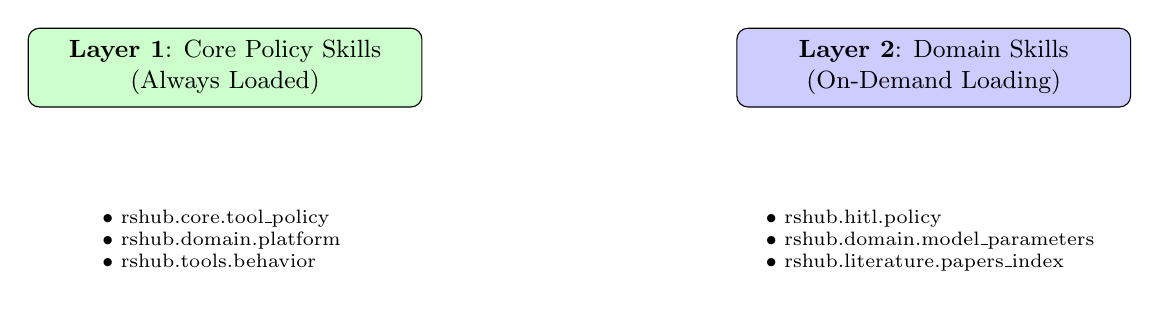
\begin{tikzpicture}[
		box/.style={rectangle, rounded corners, draw, minimum width=5cm, minimum height=1cm, align=center, font=\small}
		]
		% Increased horizontal spacing for better readability
		\node[box, fill=green!20] (l1) at (-4.5,0) {\textbf{Layer 1}: Core Policy Skills\\(Always Loaded)};
		\node[box, fill=blue!20] (l2) at (4.5,0) {\textbf{Layer 2}: Domain Skills\\(On-Demand Loading)};
		
		% Increased vertical spacing between header and item lists
		\node[font=\scriptsize, align=left] at (-4.5,-2.2) {
			\begin{tabular}{l}
				$\bullet$ rshub.core.tool\_policy\\
				$\bullet$ rshub.domain.platform\\
				$\bullet$ rshub.tools.behavior
			\end{tabular}
		};
		\node[font=\scriptsize, align=left] at (4.5,-2.2) {
			\begin{tabular}{l}
				$\bullet$ rshub.hitl.policy\\
				$\bullet$ rshub.domain.model\_parameters\\
				$\bullet$ rshub.literature.papers\_index
			\end{tabular}
		};
	\end{tikzpicture}
	\caption{Skill Tiered Loading Architecture}
\end{figure}

\subsection{Skill Definition Structure}

\begin{lstlisting}[language=YAML, caption=Skill YAML Schema, basicstyle=\ttfamily\scriptsize]
	id: rshub.hitl.policy                    # Unique identifier
	short_description: "HITL Safety Policy"   # Short description
	tags: ["core", "safety", "hitl"]          # Classification tags
	full_doc: |                             # Full documentation (Markdown)
	# HITL Safety Policy
	## Core Principles
	Any operation involving computing resources...
	bound_tool: null                        # Bound tool name (if any)
	requires_confirmation: false            # Whether confirmation required
\end{lstlisting}

\subsection{Core Skills}

\begin{longtable}{@{}p{5.5cm}p{2.8cm}p{5.2cm}@{}}
	\caption{Core Skills Inventory} \\
	\toprule
	\textbf{Skill ID} & \textbf{Loading} & \textbf{Description} \\
	\midrule
	\endfirsthead
	\multicolumn{3}{c}{\tablename\ \thetable{} -- Continued} \\
	\toprule
	\textbf{Skill ID} & \textbf{Loading} & \textbf{Description} \\
	\midrule
	\endhead
	\bottomrule
	\endfoot
	rshub.hitl.policy & On task submit & HITL four-step process and safety \\
	rshub.core.tool\_policy & Always & Tool invocation policies \\
	rshub.core.response\_guidelines & Always & Response format guidelines \\
	rshub.domain.platform & Always & Platform basic information \\
	rshub.tools.behavior & Always & Tool behavior descriptions \\
	rshub.domain.model\_parameters & On demand & Model parameter details \\
	rshub.literature.papers\_index & On demand & Scientific literature index \\
\end{longtable}

\subsection{Skill Selection Algorithm}

\begin{enumerate}
	\item \textbf{Always-on load}: inject core policy and platform skills first
	\item \textbf{HITL-aware routing}: add HITL policy/confirm skills when state or exact confirmation input requires them
	\item \textbf{Keyword routing}: include literature/model-parameter skills using deterministic pattern matching
	\item \textbf{Selective injection}: include only selected layer-2 full documents for the current turn
\end{enumerate}

% ============================================
% Section 4: Workflow and Processes
% ============================================
\section{Workflow and Processes}
\label{sec:chap4-workflow}

\subsection{Standard Task Processing Flow}

\begin{figure}[H]
	\centering
	\begin{tikzpicture}[
		startstop/.style={rectangle, rounded corners, minimum width=2.5cm, minimum height=0.7cm, text centered, draw, fill=red!20, font=\small},
		process/.style={rectangle, rounded corners, minimum width=3cm, minimum height=0.7cm, text centered, draw, fill=blue!15, font=\small},
		decision/.style={diamond, aspect=2, minimum width=1.5cm, text centered, draw, fill=orange!20, font=\scriptsize},
		arrow/.style={thick,->,>=stealth}
		]
		\node (start) [startstop] {User Request};
		\node (parse) [process, below=of start] {Intent Parsing};
		\node (react) [process, below=of parse] {ReAct Loop};
		\node (decide) [decision, below=of react] {Tool?};
		\node (hitl) [process, below left=1cm of decide] {HITL};
		\node (tool) [process, below=of hitl] {Tool Exec};
		\node (result) [process, right=2cm of tool] {Process Result};
		\node (end) [startstop, above=of result] {Response};
		\draw[arrow] (start) -- (parse);
		\draw[arrow] (parse) -- (react);
		\draw[arrow] (react) -- (decide);
		\draw[arrow] (decide) -- node[anchor=east, font=\scriptsize] {Yes} (hitl);
		\draw[arrow] (hitl) -- (tool);
		\draw[arrow] (tool) -- (result);
		\draw[arrow] (result) -- (end);
		\draw[arrow] (decide) -| node[anchor=west, font=\scriptsize] {No} (end);
	\end{tikzpicture}
	\caption{Standard Task Processing Flow}
\end{figure}

\subsection{HITL State Machine}

\textbf{States}: IDLE $\rightarrow$ PENDING\_CONFIRMATION $\rightarrow$ CONFIRMED $\rightarrow$ SUBMITTED $\rightarrow$ IDLE

\begin{table}[H]
	\centering
	\caption{HITL State Definitions}
	\begin{tabular}{@{}clp{6cm}@{}}
		\toprule
		\textbf{State} & \textbf{Name} & \textbf{Description} \\
		\midrule
		IDLE & Idle & Normal operation, no pending submission \\
		PENDING\_CONFIRMATION & Pending & Waiting for explicit confirm/cancel input \\
		CONFIRMED & Confirmed & Submit tool is allowed \\
		SUBMITTED & Submitted & Submission completed, state ready to reset \\
		\bottomrule
	\end{tabular}
\end{table}

\subsection{HITL Four-Step Process}

\begin{enumerate}
	\item \textbf{Plan}: Analyze requirements, determine tools, extract parameters
	\item \textbf{Check}: Present plan to user, explain expected results and risks
	\item \textbf{Confirm}: Wait for explicit response (\texttt{confirm/cancel}); non-matching input does not trigger submission
	\item \textbf{Execute}: Run submission only after confirmation and deduct credits only on successful submit
\end{enumerate}

\subsection{ReAct Reasoning Loop}

\begin{lstlisting}[language=Python, caption=ReAct Loop Pseudocode, basicstyle=\ttfamily\scriptsize]
	def react_loop(user_message, context):
	steps = []
	max_steps = 5
	
	while len(steps) < max_steps:
	# Thought: Analyze current state
	thought = llm.generate_thought(
	message=user_message,
	history=steps,
	skills=loaded_skills
	)
	
	if thought.intent == "direct_answer":
	return generate_response(thought)
	
	# Action: Decide next action
	action = llm.select_action(thought, available_tools)
	
	if action.type == "respond":
	return generate_response(action)
	
	# HITL Check
	if action.requires_hitl:
	hitl_result = run_hitl_flow(action)
	if not hitl_result.confirmed:
	return "Operation cancelled"
	
	# Observation: Execute tool
	observation = execute_tool(action)
	steps.append({"thought": thought, "action": action, 
		"observation": observation})
	
	if is_answer_complete(observation, user_message):
	break
	
	return synthesize_final_answer(steps)
\end{lstlisting}

% ============================================
% Section 5: API and Data Format Specification
% ============================================
\section{API and Data Format Specification}
\label{sec:chap4-api}

\subsection{API Endpoints Overview}

\begin{table}[H]
	\centering
	\caption{RESTful API Endpoints}
	\begin{tabular}{@{}llll@{}}
		\toprule
		\textbf{Endpoint} & \textbf{Method} & \textbf{Description} & \textbf{Auth} \\
		\midrule
		/api/agent/chat & POST & Send chat message & Token \\
		/api/agent/chat/stream & POST & Streaming chat (SSE) & Token \\
		/api/agent/sessions & GET/POST & List/Create sessions & Token \\
		/api/agent/sessions/{id} & GET/DELETE & Get/Delete session & Token \\
		/api/tasks/submit & POST & Submit computing task & Token \\
		/api/tasks/check & GET & Query task status & Token \\
		/api/tasks/download & GET & Get download link & Token \\
		/api/credits & GET & Query credit balance & Token \\
		\bottomrule
	\end{tabular}
\end{table}

\subsection{Key Data Models}

\subsubsection{ChatRequest}

\begin{lstlisting}[style=jsonstyle, basicstyle=\ttfamily\scriptsize]
	{
		"message": "Calculate soil moisture at 10GHz",
		"chat_id": "chat_1234567890",     // Optional
		"token": "user_jwt_token",
		"attachments": []                   // Optional
	}
\end{lstlisting}

\subsubsection{ChatResponse}

\begin{lstlisting}[style=jsonstyle, basicstyle=\ttfamily\scriptsize]
	{
		"chat_id": "chat_1234567890",
		"message": "Agent response",
		"phase": "IDLE",                    // IDLE/PENDING/CONFIRMED
		"proposed_action": {               // When confirmation needed
			"tool": "submit_rshub_task",
			"parameters": {...}
		}
	}
\end{lstlisting}

\subsubsection{TaskSubmitRequest}

\begin{lstlisting}[style=jsonstyle, basicstyle=\ttfamily\scriptsize]
	{
		"task_type": "soil",              // soil/snow/vegetation
		"model": "NMM3D",                 // Model name
		"parameters": {                   // Model-specific params
			"frequency": 10.0,
			"temperature": 300.0,
			"soil_moisture": 0.2
		},
		"token": "user_jwt_token"
	}
\end{lstlisting}

\subsubsection{HITLState Model}

\begin{lstlisting}[language=Python, basicstyle=\ttfamily\scriptsize]
	class HITLPhase(str, Enum):
	IDLE = "idle"
	PENDING_CONFIRMATION = "pending_confirmation"
	CONFIRMED = "confirmed"
	SUBMITTED = "submitted"
	
	class HITLState(BaseModel):
	phase: HITLPhase = HITLPhase.IDLE
	pending_task_spec: Optional[Dict] = None
\end{lstlisting}

\subsection{Error Codes}

\begin{longtable}{@{}llp{5cm}@{}}
	\caption{API Error Codes} \\
	\toprule
	\textbf{Error Code} & \textbf{HTTP Status} & \textbf{Description} \\
	\midrule
	\endfirsthead
	\multicolumn{3}{c}{\tablename\ \thetable{} -- Continued} \\
	\toprule
	\textbf{Error Code} & \textbf{HTTP Status} & \textbf{Description} \\
	\midrule
	\endhead
	\bottomrule
	\endfoot
	INVALID\_TOKEN & 401 & Token invalid or expired \\
	INSUFFICIENT\_CREDITS & 402 & Insufficient credit balance \\
	HITL\_TIMEOUT & 408 & Confirmation timed out \\
	INVALID\_PARAMETERS & 400 & Parameter validation failed \\
	TASK\_SUBMISSION\_FAILED & 500 & Task submission failed \\
	LLM\_SERVICE\_ERROR & 503 & LLM service unavailable \\
	RATE\_LIMIT\_EXCEEDED & 429 & Request rate limit exceeded \\
	TASK\_NOT\_FOUND & 404 & Task ID not found \\
\end{longtable}

\subsection{Environment Variables}

\begin{lstlisting}[basicstyle=\ttfamily\scriptsize]
	# Server
	HOST=0.0.0.0
	PORT=8000
	
	# RSHub API
	RSHUB_BASE_URL=https://rshub.zju.edu.cn
	
	# LLM Provider: volcengine or openrouter
	LLM_PROVIDER=volcengine
	VOLCENGINE_API_KEY=xxx
	VOLCENGINE_MODEL=deepseek-v3-2-251201
	
	# HITL
	HITL_ENABLED=true
	HITL_TIMEOUT_SECONDS=300
	
	# Billing
	TASK_SUBMIT_COST=1
	AGENT_CHAT_COST=1
	
	# CORS
	CORS_ORIGINS=http://localhost:3000,https://rshub.zju.edu.cn
\end{lstlisting}
